% !TEX root = ../Dissertation.tex
%===================================================================================================

\chapter{Discussion}

Type 1 diabetes is believed to be due to a breakdown in central tolerance of T cells in the thymus.
Using the NOD mouse as a model of T1D, it has been noted that there is an increased population of B cells found in their thymus, in comparison to non diabetes prone control B6 mice.
The origin and role of these B cells are not known.
This project aims to investigate more fully the potential intrathymic development of B cells.

Through this project, it has been confirmed that B cells are increased in the NOD mouse thymus with respect to B6 control mice, and that this increase is age-related.
In terms of potential intrathymic development, it has been shown that the thymus contains B cell development transcription factors and therefore could be conducive to B cell development.
Also, pro and pre B cells are present in the thymus of NOD mice, though the population frequency appears to be dependent on the presence of a mature B cell.
Further to this, there is evidence of active B cell receptor rearrangement in the thymus indicative of active B cell development.
However, the progenitor from which thymic B cells are originating from is less clear. 
Whilst BLPs are present in both NOD and B6 mouse thymi, they are significantly decreased in the NOD mouse compared to B6 mouse suggesting an alternative progenitor for thymic B cells, at least in the NOD mouse.

Also, further to these findings, there were some interesting results which suggested the presence of a cell in the thymus expressing markers of both T and B cells, and in fact a small population expressing both a B and T cell receptor.
These could provide an alternative mechanism for B cell development through re-differentiation of T cells.


\section{There is an age-related increase in thymic B cells in the NOD mouse}

The results showing an age-related increase in thymic B cells in the NOD mouse compared to the B6 control mouse suggests there may be a correlation between thymic B cells and T1D progression.
T1D onset occurs with initial priming of T cells between 3-5 weeks of age. 
At this point there is autoimmune response and the population of B cells in the NOD thymus is not increased compared to control B6 mice.
However, by 9 weeks of age, this is when the islets of the NOD mouse become infiltrated and in the thymus, B cells start to increase with respect to those seen in the B6 control mice.
By 12 weeks, immune cells in the islets of the NOD mouse become aggressive and $\beta$ cells are destroyed. 
This correlates with a further significant increase in B cells in the NOD mouse thymus compared to the B6 mouse thymus.

T cell development and education occurs within the thymus, in particular the first step of T cell tolerisation, negative selection.
This is where autoreactive T cells are purged from the repertoire to prevent potential autoimmunity.
T1D is believed to be due to a breakdown in tolerance and therefore it may be that B cells found in the thymus of NOD mice may be contributing to this process.
There is evidence that B cells are able to contribute to the process of negative selection, as shown by the likes of \toref{} and \toref{} etc who have shown that.... \todo{Add in the papers of who did what lookign at thymic B cells in nagative selection}

Supposing thymic B cells are having an affect on negative selection, it is not known if their contribution is useful in aiding removal of autoreactive developing T cells, or a hindrance to their deletion.
It could also be that instead of being a driving force in the breakdown of negative selection, they may be a consequence, such that their development is triggered to help with an increasing population of developing autoreactive T cells.
\citet{Yamano2015} have shown that some thymic B cells are able to express AIRE in AIRE-reporter mice. \todo{Yamano, what did they do? Tolerogenic features of thymic B cells?}
Whilst this is in mouse not of the NOD background, it does suggest a potential useful role of thymic B cells which may or may not be applicable to the NOD mouse.

\section{B cells are developing intrathymically}

\subsubsection{Thymic pro and pre B cell presence}
The main hypotheses for the origins of thymic B cells are intrathymic development from progenitors and migration of B cells from the bone marrow to the thymus.
The general consensus is that B cells are developing within the thymus with very little contribution from the circulation.
Experiments involving parabiotic congenic mice showed that of the thymic B cells, the majority were of the endogenous phenotype, not the parabiotic partner. 
This gave the impression that the thymic B cells have more to do with the thymus itself, rather than the circulation \citep{Perera2013}.
Similarly, \citet{Akashi2000} found that when donor B cells of a different Ly5 isoform were injected into recipient mice, very few of the thymic emigrant B cells were of donor origin, suggesting that they could be more attributable to development within the host rather than a result of circulating B cells stopping in the thymus.

This project aimed to further investigate this intrathymic development and the evidence from the data shown agrees with the hypothesis of intrathymic B cell development.

Firstly, pro and pre B cells were investigated in the thymus of both NOD and B6 mice. 
This is similar to the findings of both \citet{Hashimoto2002} and \citet{Akashi2000} who both showed presence of pro B cells in the thymus of mice.
However, the mice they were using were not prone to T1D or any autoimmunity therefore their findings may or may not be applicable to mice of the NOD background.
\citet{Hashimoto2002} also showed an interesting finding that in BALB/cJ mice, there was .... something to do with IL-7.
Il-7 is important for B cell development \citep{Corfe2012}.
The presence of pro and pre B cells in the thymus suggests that B cells may be developing there as they are two fundamental stages of normal B cell development.

Interestingly, it appeared that the frequency of the thymic pro B cell population is dependent on whether or not mature B cells are present.
That is, in NOD KO mice, the frequency of thymic pro B cells was reduced compared to in both NOD and B6 mouse thymi.
This result was not expected and begs the question as to how to investigate this further.
Some potential roles of a mature B cell include the following.
\begin{itemize}
\item A mature B cell may be helping with the recruitment of B cell progenitors from the bone marrow to the thymus
\item A mature B cell may provide a survival factor for B cell progenitors within the thymus so that they survive to be able to develop
\item A mature B cell may kick start the process of B cell transcription factor expression within the thymus, so that the thymus can provide an environment conducive to B cell development
\item A mature B cell may provide a survival factor for newly developed B cells so that once they have developed they are able to survive.
\end{itemize}

Of course, an obvious potential method for further investigation would be to transfer mature B cells from a B cell sufficient NOD mouse into the NOD KO mouse to see if these donor B cells can have an effect on the thymic pro B cell population.
However, a pilot study of this method was attempted and showed that the donor B cells did not survive to 11 days post transfer.

This transfer approach has also been attempted by \citet{Serreze1998} where mature splenic B cells were transferred into NOD KO recipient mice and a similar finding was observed in that the B cells disappeared between 6 and 11 days post transfer.
\citet{Serreze1998} showed that this disappearance was due to CTL destruction of the donor B cells, presumably due to the lack of B cell presence during endogenous T cell development therefore the T cells would never have been tolerised to B cells.

However, it is not known if this is also the case in the transfer experiment shown in this project.
It is not known if CTL mediated B cell destruction was also occuring in this transfer utilising thymic B cells (rather than splenic), or whether it was a different mechanism causing their disappearance. 
If CTL mediated destruction is the cause, it would be of interest to know where this killing was taking place. 
For example, B cells were seen in both the spleen and thymus at the 7 day post transfer time point.
Therefore, unless B cells that have reached these tissues leave again and are then destroyed, it suggests that CTL activity may be happening within the thymus and spleen. \todo{Is this strange? where do CTLs act?}

The fact that this approach appears to be inappropriate to determine the effects of mature B cells on thymic pro B cell populations means that an alternative approach must be found.
\citet{Serreze1998} continued investigations by irradiating recipient mice then transplanting NOD KO bone marrow supplemented with NOD B cells.
This results in endogenous effector immune cells developing in the presence of B cells and should avoid the T cell destruction of donor B cells.
This could therefore be a way forward to investigate the effect of B cells on the population of pro B cells in the NOD KO thymus.
By adding purified mature B cells, it would be interesting to see if this was sufficient to increase pro B cell frequency in the KO thymus.
Following this, it would also be of interest to try transplanting KO bone marrow supplemented with B6 B cells to see if it is a characteristic of a NOD B cell that can increase thymic pro B cells.
It is not known whether the mature B cell needs to be of splenic or thymic origin, therefore these experiments could also test that by separately transferring bone marrow supplemented with B cells from both tissues.

\subsubsection{BcR rearrangement in the thymus}


For pro B cells to progress to the pre B cell stage, the IgM heavy chain must be rearranged.
Therefore, it was wondered whether the thymus is able to support this developmental step.
To tackle this question, RAG expression was looked for in CD19\textsuperscript{+} cells in the thymus of NOD mice.
It was seen that there are populations of CD19\textsuperscript{+}RAG\textsuperscript{high}, CD19\textsuperscript{+}RAG\textsuperscript{low} and CD19\textsuperscript{+}RAG\textsuperscript{-} cells in the NOD thymus.
The RAG\textsuperscript{high} cells are very likely developing there within the thymus as this very bright signal was equivalent to that seen in actively developing T cells in the thymus.
This gives the impression that RAG is being actively transcribed in CD19\textsuperscript{+} cells in the thymus, indicating active BcR rearrangement and B cell development.

These RAG expressing CD19\textsuperscript{+} cells were looked for in NOD-RAG-GFP mice of 4, 7 and 11 weeks of age and interestingly, the CD19\textsuperscript{+}RAG\textsuperscript{high} population frequency didn't change, whereas the CD19\textsuperscript{+}RAG\textsuperscript{low} frequency decreased significantly.
This gives the impression that as mice age, there are less newly developed B cells in the thymus, potentially as a result of decreased development.
This decrease suggests that the development of B cells within the thymus may be restricted to younger mice and that that intrathymic B cell development may be deactivated at a certain time point in the disease process.
However, it may be that more newly developed B cells are leaving the thymus in older mice compared to younger ones so that the population of newly developed B cells within the thymus is decreased.

If the decrease in CD19\textsuperscript{+}RAG\textsuperscript{low} cells is due to a decrease in development, this may be due to the fact that within the thymus there are multiple different niches harbouring different types of cells.
It may be that the downregulation of B cell development occurs as a result of the B cell niche (if one exists) becoming too full \todo{Thymic niches}.
Further to this, thymi atrophy with age, therefore a thymus which is decreasing in size would have less space available for cells to reside in, including B cells, so it may be that with increasing age, B cell development is decreased. \todo{Age-related thymic atrophy}

On the other hand, if newly developed B cells are leaving the thymus and travelling elsewhere, it may be that the thymus is acting like the bone marrow, harbouring B cell development then allowing their release to mature in a different tissue, such as the spleen.

However, neither of these suggestions account for the overall picture of an increase in B cells in the NOD mouse thymus compared to the B6 mouse thymus.
It does, however, suggest that the increased population of thymic B cells may not be directly linked to the rate of B cell development, but more to proliferation of developed B cells.

In this case, it may be that the thymus is acting like the bone marrow, harbouring B cell development then releasing immature B cells to continue development elsewhere.
The decrease also coincides with disease progression, therefore it may be that thymic B cells can contribute to the process of insulitis and move to the islets.
However, this is just speculation.
It would be beneficial to track thymic cells in order to see whether they stay within the thymus or move elsewhere.

\todo{Future}

\subsubsection{BLPs are present in the NOD thymus}


It was wondered whether Sca-1\textsuperscript{low}c-kit\textsuperscript{low}Flt3\textsuperscript{+}IL-7R$\alpha$\textsuperscript{+}Ly6D\textsuperscript{+} B cell progenitors (BLPs) would be present in the NOD thymus and, if so, if they are increased in the NOD mouse compared to the B6.
When looking for potential TSPs, cells with the correct markers to allow homing were considered \citep{Zlotoff2011}, therefore, it may be that if marker expression in the bone marrow is abherrent on B cell progenitors, it may result in an excess of B cell precursors being able to migrate to the thymus alongside T cell progenitors.
For example, it would be of interest to see how the levels of Flt3, CCR7 and CCR9 expression compared between bone marrow BLPs and BLPs found in the thymus.
It may be that some express excess levels of these markers which allow B cell progenitors to migrate to the thymus along with TSPs.

It was interesting when investigating the presence of BLPs that the frequency of BLPs in the Sca-1\textsuperscript{low}c-kit\textsuperscript{low}Flt3\textsuperscript{+}IL-7R$\alpha$\textsuperscript{+} population of the thymus of the NOD mouse, was significantly decreased compared to the B6.
This was surprising due to the increased population of B cells seen in the NOD thymus compared to that of the B6.

However, before any assumptions can be made on this data, it is first necessary to consider the model of B cell development from BLPs.
For example:
\begin{itemize}
\item Are BLPs the sole progenitor for B cell development? There is evidence to suggest that this is a progenitor that is restricted to the B cell lineage, however, it is not clear if this is the only progenitor capable of differentiating into a B cell.
\item Is the B cell developmental pathway the same in the thymus as the bone marrow? The B cell development pathway in the bone marrow has been investigated extensively, however, the pathway in the thymus is much less well understood therefore whether the bone marrow development pathway can be applied to the thymus is not known. 
\end{itemize}

In order to help determine the answers to the questions above, it would be necessary to carry out further experiments.
To determine whether B cells can develop from BLPs in the thymus, it would be interesting to culture BLPs on thymic stromal cell lines, such as \todo{Thymic stromal cell lines used to culture cells, eg T cells. Or that used to culture BLPs in Inlay et al}.
This in vitro approach may be able to indicate whether or not B cells could develop from BLPs in the thymus.
However, it is unlikely that B cell development from BLPs is restricted only to the bone marrow, shown by the presence of BLPs in the B6 thymus.
These may be the origin of the normal, small population of B cells in the B6 thymus.

However, the NOD thymus has a significantly smaller frequency of BLPs in the thymus compared to the B6.
Despite this, NOD mice still have increased thymic B cells suggesting that there are different mechanisms in the NOD mouse which increase thymic B cells that are not present in the B6 mouse.

Interestingly, when comparing NOD and NOD KO thymic BLPs, there was no difference observed in the population frequency.
This means that if a mature B cell is having an effect on the pro B cell population, it's action must be after the formation of the BLP (since BLP frequency is unaffected in NOD KO mice compared to NOD mice) and prior to the formation of the pro B cell.
For this reason, it would be of interest to investigate stages between these two cells, such as pre-pro B cells, to see whether they are affected by the presence/absence of mature B cells and to try and pinpoint the time point when mature B cells have their effect.

\subsubsection{T cells may be becoming B cells}

To understand another potential mechanism for increased thymic B cells, the finding of RAG\textsuperscript{+}CD19\textsuperscript{+}CD4\textsuperscript{+}CD8\textsuperscript{+} cells in the thymus needs to be considered.
There are a few potential hypotheses about these cells, but one in particular is of interest for the increased thymic B cells seen in the NOD mouse.

These cells expressing markers of both T and B cells suggest that there may be an extra stage of normal development whereby developing T or B cells express markers of the other.
On the other hand, this process is unlikely to be a normal part of either developmental pathway due to the absence of these cells in the bone marrow (therefore unlikely to be a part of B cell development) and the fact that T cells are committed to the T cell lineage at the DN stage (prior to CD4 and CD8 expression).

It is therefore worth considering whether it is a normally developing T cell which is late to commit to the T cell lineage and is retaining some characteristics of B cells (CD19), or indeed a cell which is developing with characteristics of both T and B cells.
However, this is unlikely due to the very small prevalence of cells in the thymus that have progressed to expressing both a T and B cell receptor and are IgM\textsuperscript{+}TcR$\beta$\textsuperscript{+}.

Another possibility which could then contribute to the B cell population in the thymus is that these cells are the midpoint of a T cell transitioning to a B cell (or vice versa).
This would account for there only being a very small population of IgM\textsuperscript{+}TcR$\beta$\textsuperscript{+} cells, and the expression of both T and B cell markers.
It may also account for the decreased BLPs in the NOD compared to B6 as B cells developing from T cells would not develop originally from BLPs.
To investigate this possibility, it may be of use to look at the relative levels of B and T cell transcription factors Pax5 and Notch1.

Maintaining the correct balance of transcription factors is very important for development of lymphocytes. \todo{Koch2001 is a paper showing importance of Notch 1 in stopping B cell development}
For example, as mentioned in \cref{subsec:Bcellgenes}, it was pointed out that Pax5 expression is important for repressing T cell lineage commitment through the repression of Notch1 \citep{Souabni2002}.
It is also thought that T cells only commit to the T cell lineage and lose B cell potential once progenitors arrive in the thymus \citep{Heinzel2007}.
Further to this, Notch1 deficiency led to a loss of developing T cells and an increase thymic B cells \citep{Feyerabend2009}.
However, Notch1 is not the only important transcription factor that needs to be kept in balance.
As mentioned in \cref{subsec:Tcellgenes}, Gata3 is an important transcription factor for T cell development which requires repression by EBF for B cell development to occur \citep{Banerjee2013}.
All this just goes to show the importance of transcription factor balance.
It may be that in the thymus of NOD mice, an imbalance in transcription factor expression may be causing the excess B cell population.
Of particular interest would be Notch1 expression.
Quantitative PCR would be a way of looking at this and then a comparison could be made between normal B6 mice thymi and NOD mice thymi.
It may that there is an imbalance in the presence of transcription factors which is allowing the development of the wrong lymphocytes, or the dedifferentiation of one to the other \citep{Cobaleda2007}.

\todo{Could you isolate the cells that are RAG+CD19+CD4+CD8+ and see what they become???
Isolate, label and re-inject?
Isolate and culture?}



\section{Summary}

B cells normally develop in the bone marrow, as shown in \cref{fig:summarydiagram2}.
T cells normally develop in the thymus from CCR7/9\textsuperscript{+} LMPPs or CLPs which migrate to the thymus to become TSPs.

However, the NOD mouse has an increased population of B cells in the thymus and this project has been investigating the potential intrathymic development of these B cells.
It appears that this increase is dependent on the presence of a mature B cell.

Firstly, the potential for following the same developmental pathway of B cell development in the thymus as in the bone marrow was investigated (\cref{fig:summarydiagram2}, blue arrows).
Whilst pro and pre B cells were seen (not shown), RAG expression was seen, suggesting active B cell development.
However, the frequency of BLPs in the NOD thymus was significantly reduced compared to the B6 controls, suggesting that BLPs are not the origin for the increased thymic B cell population.
It was then considered whether there is another mechanism for intrathymic B cell development.
The potential for T to B cell transition was considered after finding a population of cells that were RAG\textsuperscript{+}CD19\textsuperscript{+}CD4\textsuperscript{+}CD8\textsuperscript{+} and therefore expressing both T and B cell markers (\cref{fig:summarydiagram2}, red arrow).
These cells could either be the midpoint of transitioning, or they may be a new type of cell in the thymus (\cref{fig:summarydiagram2}, purple arrows).
Further evidence for intrathymic B cell development is the presence of B cell development transcription factors.
Thymic B cells may be contributing to insulitis in T1D, or they may be having an effect on T cell negative selection in the thymus (\cref{fig:summarydiagram2}, black dashed arrows).
Negative selection may also be being influenced by autoantibodies (Not shown).

In T1D, healthy islets become infiltrated before the $\beta$ cells are destroyed by CTLs allowing T1D progression.


\begin{figure}
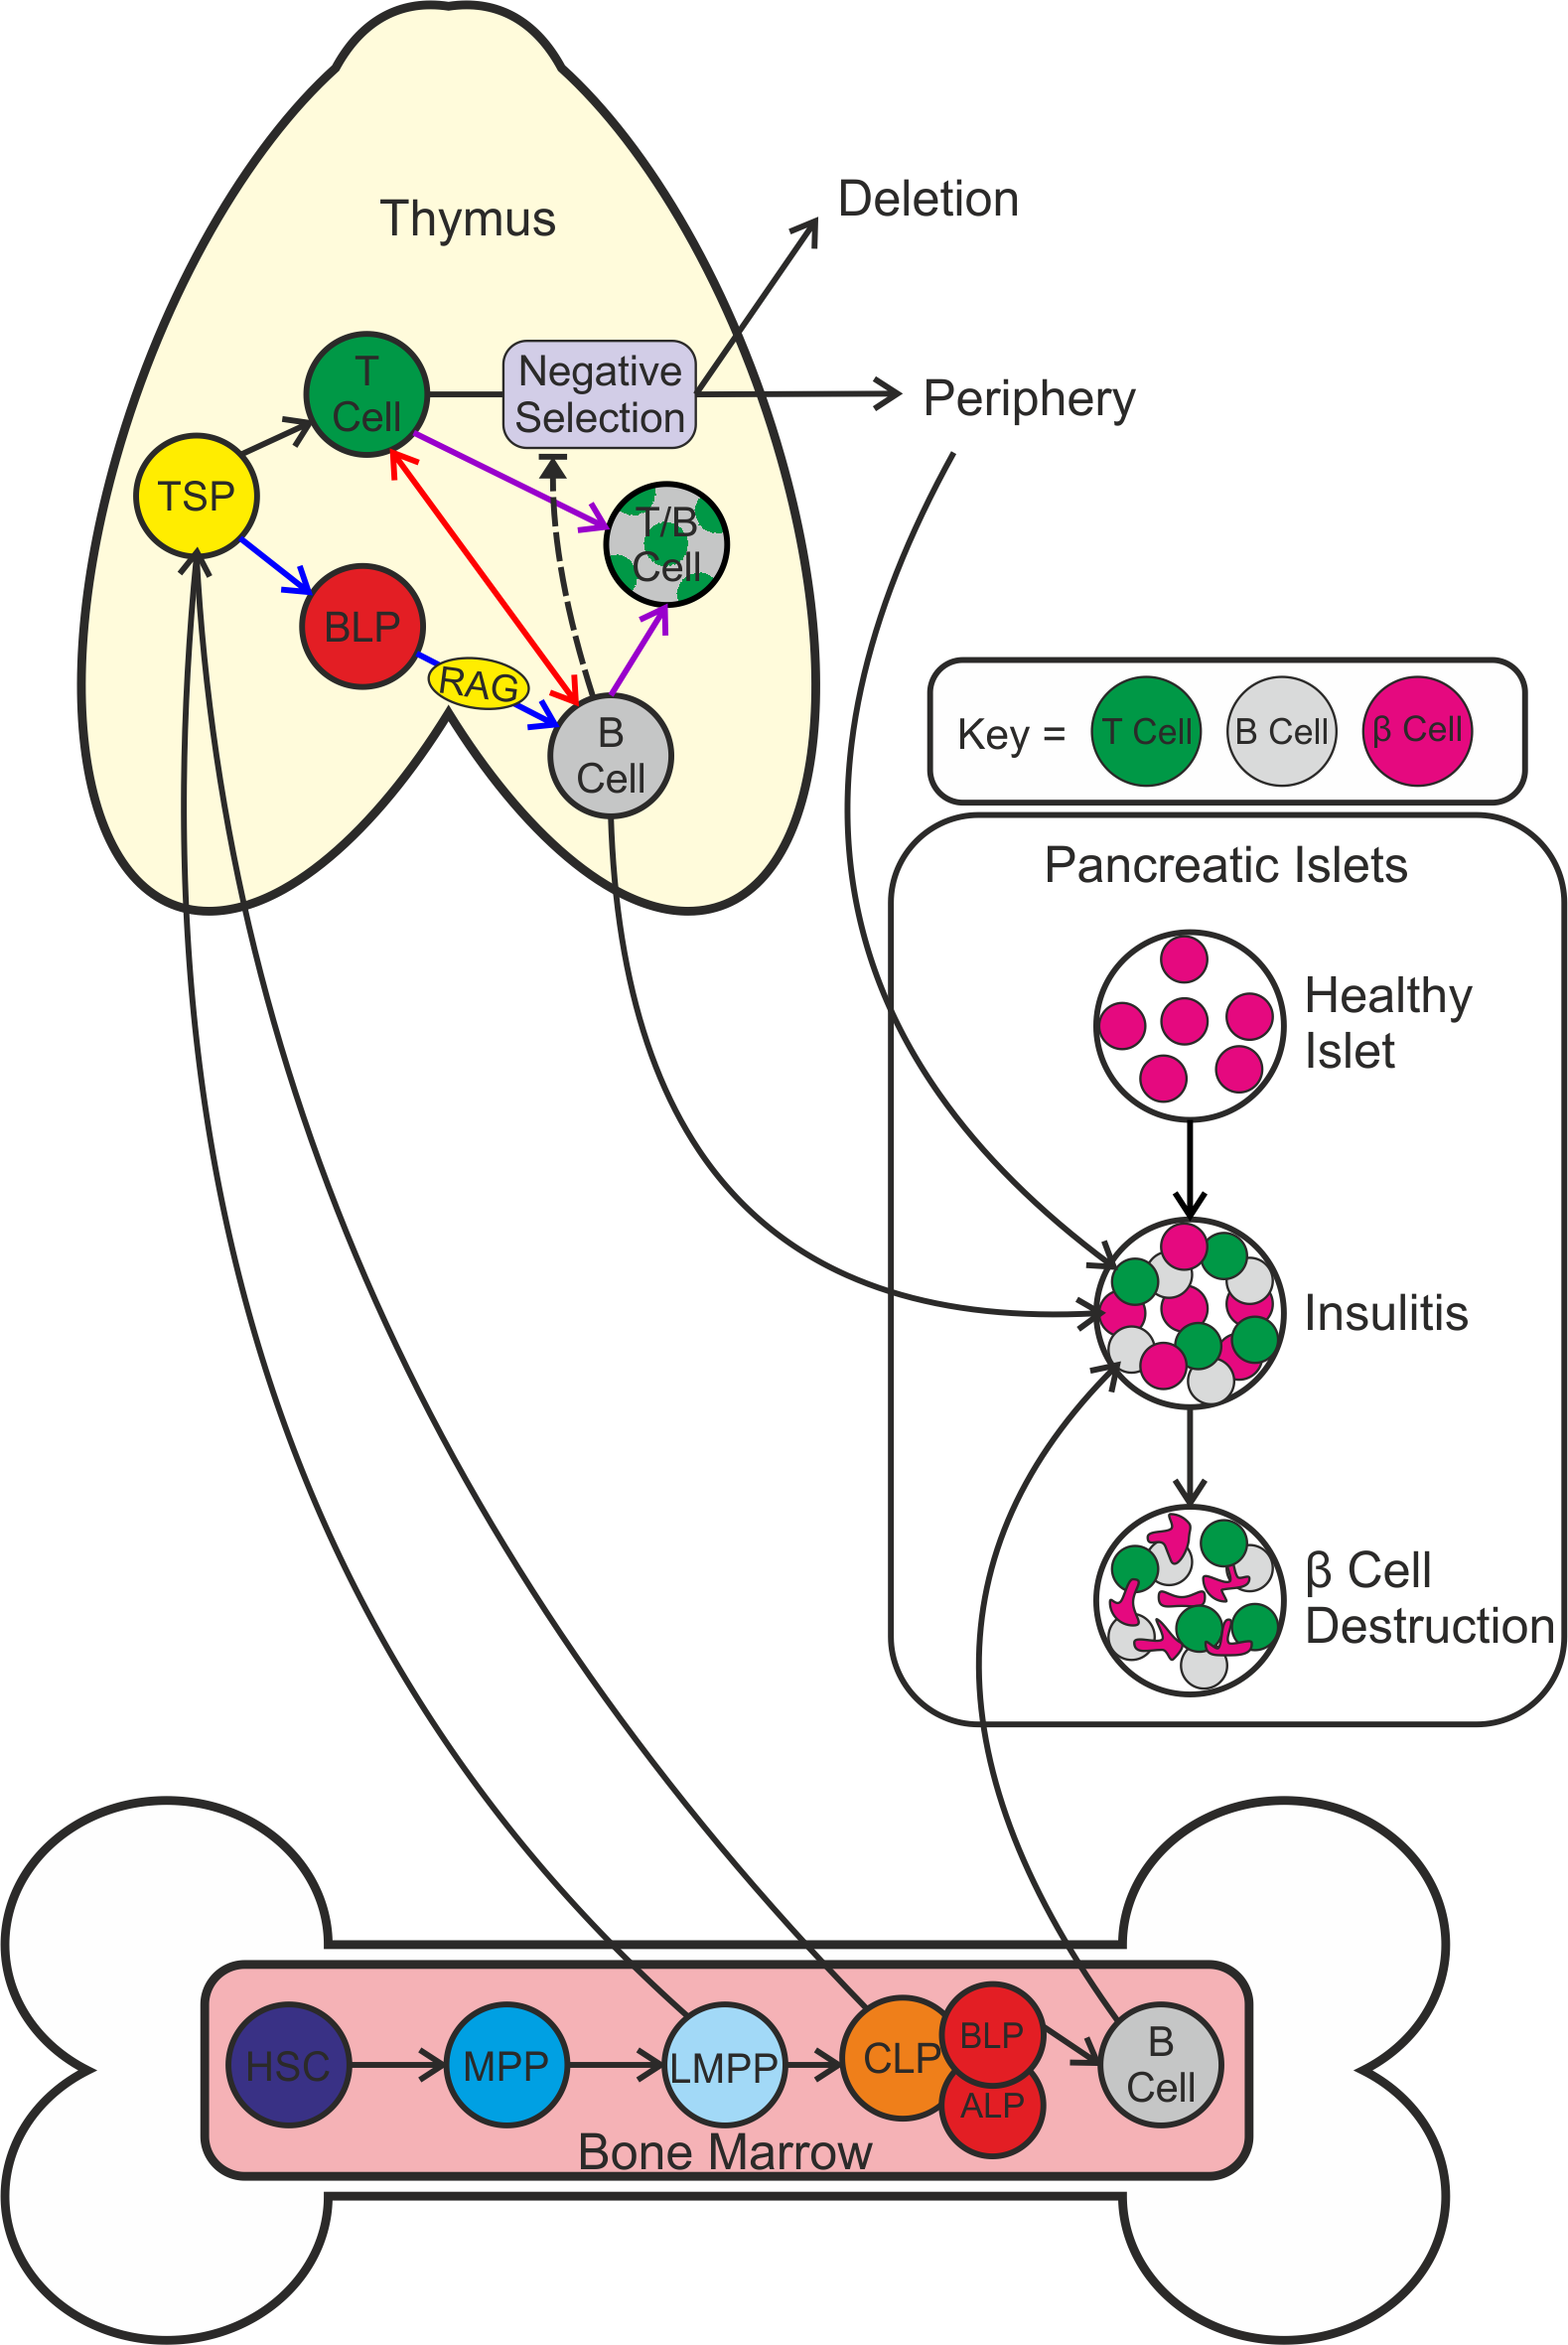
\includegraphics[width=\textwidth]{Figures/diagram2.png}
\caption[Diagrammatical summary of the project findings]{ 
B cells develop in the bone marrow. 
T cells develop from thymic settling progenitors believed to be Flt3\textsuperscript{+}CCR7/9\textsuperscript{+} LMPPs or CLPs which migrate to the thymus.
Here they develop into T cells and pass through negative selection, for which the outcome is either clonal deletion or release into the periphery.
B cells may also be developing in the thymus, either following the same pathway as seen in the bone marrow (bone marrow), or from T cells developing into B cells (red arrows).
There also appears to be evidence of a cell expressing both T and B cell markers which may arise from a B or T cell that has been triggered to display both markers (purple arrows), or may be the mid point of a transitioning T or B cell.
Thymic B cells may contribute to insulitis.}
\label{fig:summarydiagram2}
\end{figure}

















